\begin{chapter}{Jacobian algebras from polygonal subdivisions}
We have now introduced all of the definitions and tools needed to start studying Jacobian algebras arising from triangulations of surfaces. Perhaps the simplest invariant one can study is their dimension. As shown in \cite{Lad12}, all Jacobian algebras arising from surfaces with empty boundary are finite-dimensional, with perhaps the exception of the sphere with 4 punctures, which is not discussed. 

One may ask if the result does not hold in that case or if only Ladkani's proof does not apply but the result holds nevertheless. We start off studying the tetrahedron, which is a \emph{nice} triangulation of the sphere with 4 punctures, in the sense that it does not involve self-folded triangles and determine that its associated Jacobian algebra is infinite-dimensional.

We then introduce a procedure to generate a QP, and correspondingly a Jacobian algebra, from an arbitrary polygonal subdivision of a surface. We find that in this situation, there are both infinite families of subdivisions with finite-dimensional Jacobian algebra and infinite families with infinite-dimensional ones, so the situation is considerably more complicated than in the triangulated case.

Another result from \cite{Lad12} states that in the triangulated setting the finite-dimensionality of the Jacobian algebra does not depend on the choice of scalars for the potential. As we will show in this section, this does not generalize to the polygonal case.

Finally, we will make use of the diamond lemma to produce confluent rewriting system for three families of polyhedra: pyramids, prisms and antiprisms. These examples will be further studied in the next section.

\begin{section}{The tetrahedron}
\label{tetra}
We start by constructing the quiver associated to the tetrahedron, which looks like this:
\[
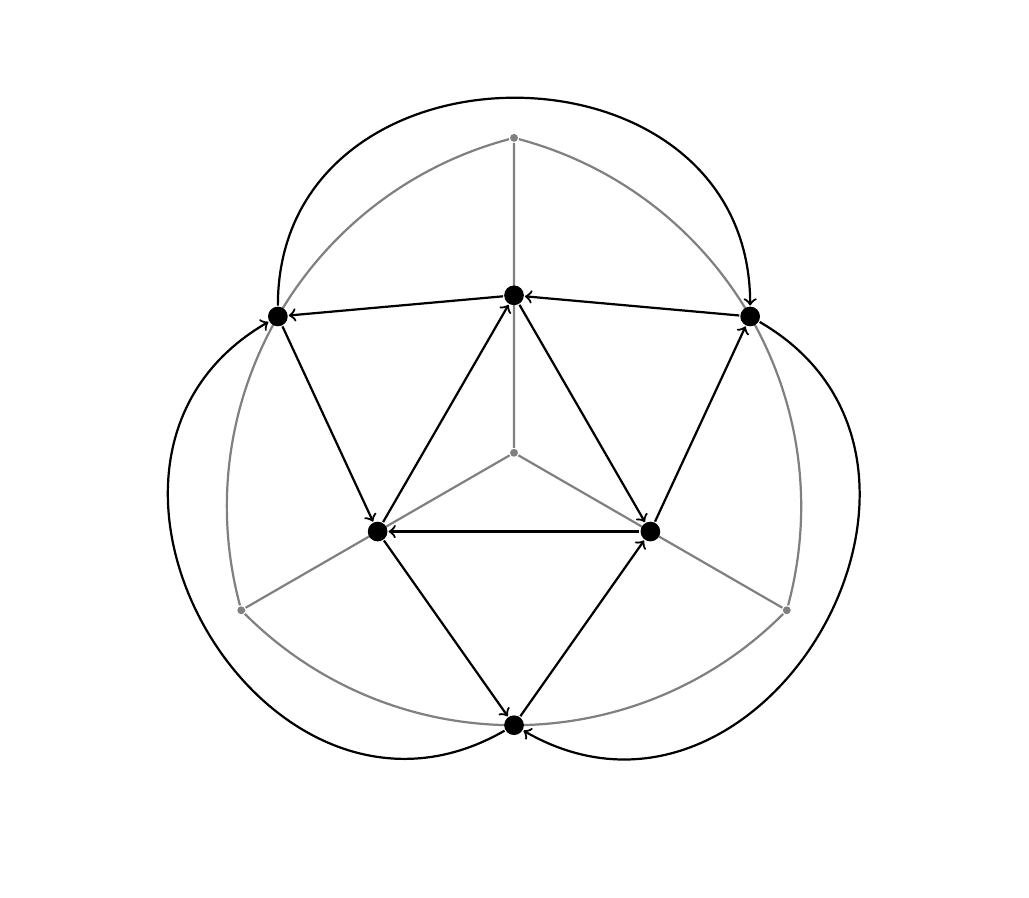
\begin{tikzpicture}[thick]
\tikzstyle{every node} = [circle, fill=gray, minimum size=.1cm, inner sep=0cm]
\node (c) at (0,0) {};
\node (n) at (0,4) {};
\node (sw) at (210:4) {};
\node (se) at (330:4) {};
\draw[gray] (c) -- (sw)
	(c) -- (n)
	(c) -- (se)
	(sw) to [bend right = 45] coordinate[midway](m1) (se)
	(n) to [bend right = 45] coordinate[midway](m2) (sw)
	(se) to [bend right = 45] coordinate[midway](m3) (n);
\tikzstyle{every node} = [circle, fill=black, minimum size=.25cm, inner sep=0cm]
\node (in) at (0,2) {};
\node (isw) at (210:2) {};
\node (ise) at (330:2) {};
\node (os) at (m1) {};
\node (onw) at (m2) {};
\node (one) at (m3) {};
\draw[->] (in) -- (onw);
\draw[->] (onw) -- (isw);
\draw[->] (isw) -- (in);
\draw[->] (in) -- (ise);
\draw[->] (ise) -- (isw);
\draw[->] (ise) -- (one);
\draw[->] (one) -- (in);
\draw[->] (isw) -- (os);
\draw[->] (os) -- (ise);
\draw[->] (one) to [bend left=90, distance=100] (os);
\draw[->] (onw) to [bend left=90, distance=100] (one);
\draw[->] (os) to [bend left=90, distance=100] (onw);
\end{tikzpicture}
\]
In the figure, the edges of the triangulation are gray, while arrows in the quiver are black. The outermost 3-cycle corresponds to the bottom face of the tetrahedron. We observe that this quiver appears in {\cite{VD14}*{Example 1.4.4}}, as an example of what the author calls a quiver with an infinite \emph{cyclic sequence}. The potential, as we may recall from \hyperref[qp]{Section \ref*{qp}}, is the sum of the four 3-cycles coming from the triangular faces of the tetrahedron and the four 3-cycles around each puncture of the sphere.

While this triangulation is very simple, studying its associated Jacobian algebra can be quite troublesome. Our strategy is to name all arrows, sort paths using the revglex order and try to apply the diamond lemma in order to produce a basis for it. However, the fact that there are 12 edges in the quiver makes calculation by hand difficult. Since every edge induces a different cyclic derivative, and therefore a different relation in the Jacobian algebra, we have 12 rewriting rules that overlap themselves in various ways. It is not clear at all if the system is confluent or not, and checking that would imply a sizeable number of verifications. Moreover, if it turns out \emph{not} to be confluent, we may apply \hyperref[heuristic]{Heuristic \ref*{heuristic}} as to enlarge the rule set and try to achieve confluence, but this only increases the number of verifications one needs to perform.

The problem is then too large to deal with by hand, but it looks reasonable enough to try to solve it using a computer. Perhaps the most suitable existing software package for this is \texttt{bergman} (freely available at \url{http://servus.math.su.se/bergman/}), which is a general purpose Gröbner basis calculator for the non-commutative setting. However, while \texttt{bergman} operates with arbitrary quotients of free algebras, we are dealing with a very specialized problem: our algebra is a quotient of a complete path algebra. Imitating the process we described in \hyperref[path-diamond]{Section \ref*{path-diamond}}, we can present complete path algebras as quotients of the completion of free algebras, but this introduces a huge number of relations that greatly slows down computation. Thus it makes sense to program our own piece of software to deal with this particular situation.

We chose \texttt{SageMath} (freely available at \url{http://www.sagemath.org/}) as a framework to develop our program, since it has an extensive general purpose library. On a more particular note, it also includes a comprehensive directed graphs library that makes it easier for us to input and work with our quiver.

A description of our algorithms and the code itself are presented in detail in \hyperref[appendix]{Appendix \ref*{appendix}}. We will now make use of our software to study the Jacobian algebra associated to the tetrahedron.

We start by inputting our triangulation; the program will then produce the associated QP, label the vertices of the quiver and then generate the rewriting system induced by the revglex order. Then, the system will be tested for confluence and, if that is not the case, will enlarge the set of rules as described in \hyperref[heuristic]{Heuristic \ref*{heuristic}} until confluence is achieved. The output reads:
\begin{lstlisting}
sage: tetrahedron = Rewriting_System(graphs.TetrahedralGraph())
Total rules: 12
\end{lstlisting}
As we anticipated, there are 12 rewriting rules, but the program finishes its execution without adding more of them, which means the obvious rewriting system is indeed confluent. We now display the labeling of the vertices of the quiver the program used:
\begin{lstlisting}
sage: tetrahedron.quiver.show()
\end{lstlisting}
The output of this line of code is shown on \hyperref[quiverfigure]{Figure \ref*{quiverfigure}}.
\begin{figure}[h] \label{quiverfigure}
\centering
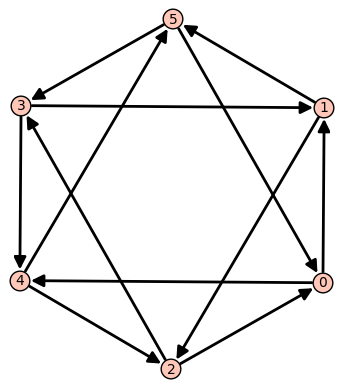
\includegraphics[width=0.5\textwidth]{tetra_quiver.png}
\caption{}
\end{figure}
Notice that it is exactly the same quiver as we have drawn before. We will call it $Q$. Let us now display the set of rewriting rules produced:
\begin{lstlisting}
sage: tetrahedron.rules
{(0, 2, 1): -(0, 3, 1),
 (0, 2, 4): -(0, 3, 4),
 (1, 0, 2): -(1, 5, 2),
 (1, 0, 3): -(1, 5, 3),
 (2, 1, 0): -(2, 4, 0),
 (2, 1, 5): -(2, 4, 5),
 (3, 1, 0): -(3, 4, 0),
 (3, 1, 5): -(3, 4, 5),
 (4, 0, 2): -(4, 5, 2),
 (4, 0, 3): -(4, 5, 3),
 (5, 2, 1): -(5, 3, 1),
 (5, 2, 4): -(5, 3, 4)}
\end{lstlisting}
Paths are described as lists of vertices, meant to be read from left to right. For example, $(0,2,1)$ is the path of length 2 obtained by concatenating the arrow with source 0 and target 2 to the arrow with source 2 and target 1. Rewriting rules are described as pairs of paths, where the leftmost path is the one that is replaced by the rightmost. For instance, following our previous notation, the rule $(0, 2, 1): -(0, 3, 1)$ may be represented as $(0,2,1) \rightsquigarrow -(0,3,1)$.

Since the rewriting system is confluent, a basis for the Jacobian algebra is given by the set of irreducible paths, which are exactly the ones that do not contain any of the 12 paths that appear in the left side of the rewriting system. We will now draw a different quiver, called $Q'$, having the arrows of our old quiver as vertices and we will place an arrow joining two of them if the path of length 2 formed by concatenating those arrows is irreducible:

\[
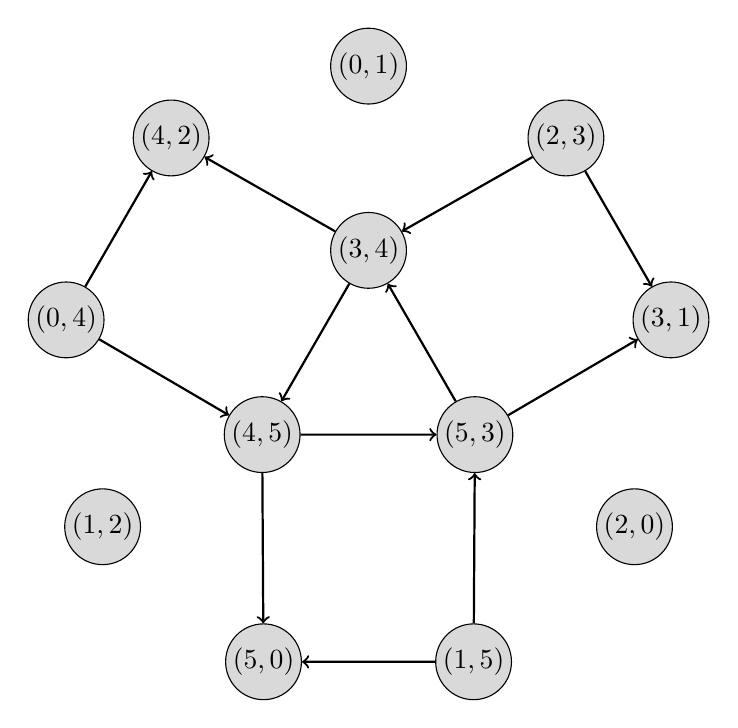
\begin{tikzpicture}[->, thick, scale=1.3]
\tikzstyle{every node} = [circle, fill=gray!30, minimum size=.5cm, inner sep=.04cm, draw=black, thin]
\node (1) at (90:1.2) {$(3,4)$};
\node (2) at (210:1.2) {$(4,5)$};
\node (3) at (330:1.2) {$(5,3)$};
\node (4) at (10:3) {$(3,1)$};
\node (5) at (50:3) {$(2,3)$};
\node (6) at (130:3) {$(4,2)$};
\node (7) at (170:3) {$(0,4)$};
\node (8) at (250:3) {$(5,0)$};
\node (9) at (290:3) {$(1,5)$};
\node (10) at (90:3) {$(0,1)$};
\node (11) at (210:3) {$(1,2)$};
\node (12) at (330:3) {$(2,0)$};
\tikzstyle{every node} = []
\draw (1) -- (2);
\draw (2) -- (3);
\draw (3) -- (1);
\draw (3) -- (4);
\draw (5) -- (4);
\draw (5) -- (1);
\draw (1) -- (6);
\draw (7) -- (6);
\draw (7) -- (2);
\draw (9) -- (8);
\draw (9) -- (3);
\draw (2) -- (8);
\end{tikzpicture}
\]

Any path in this new quiver represents a path in the original quiver $Q$ obtained by concatenating irreducible paths of length 2. Now, since the rewriting rules affect paths of length 2 only, we see that any path in the new quiver $Q'$ represents an irreducible element in the Jacobian algebra. As $Q'$ is not acyclic, we conclude that there are an infinite number of irreducible elements, and therefore the Jacobian algebra is infinite-dimensional.

In fact, we can calculate a finer invariant. Given a graded algebra $A=\bigoplus_{n=0}^\infty A_n$, its \emph{Hilbert series} $h_A(t)$ is the ordinary generating function induced by the sequence $(\dim_k(A_n))$. In other words,
\[h_A(t) = \sum_{n=0}^\infty \dim_k(A_n)\,t^n.\]
Any path algebra is obviously graded by path length. Now, the Jacobian algebra associated to the tetrahedron (which we will call $A$ for the remainder of this section) is a quotient of a path algebra by an \emph{homogeneous} ideal, since the Jacobian ideal is generated by the 12 homogeneous binomials of degree 2 given by the rewriting rules shown above. Therefore, the original grading of the path algebra passes to the quotient and so $A$ itself is graded. 

In the light of this fact, it makes sense to calculate its Hilbert series. We know that a basis for the homogeneous component of degree $n$ of $A$ is given by the set of irreducible paths of length $n$, so we just have to count them. Since the rewriting rules involve paths of length 2 only, all paths of length 0 and 1 are irreducible, and so $\dim_k(A_0)=6$ (the number of vertices in $Q$) and $\dim_k(A_1)=12$ (the number of arrows in $Q$). We know that $\dim_k(A_2)=12$ as well, since this is the number of arrows in the quiver $Q'$. In general, for $n\geq 3$, there are as many irreducible paths of length $n$ in $Q$ as paths of length $n-1$ in $Q'$. An easy counting argument shows that there are exactly 12 of them for all $n\geq 3$, since there are exactly 2 of them starting at each of the vertices $(0,4),(1,5), (2,3), (3,4), (4,5)$ and $(5,3)$ and none starting at any other vertices. Therefore, we conclude that the Hilbert series is
\[h_A(t)=6+\sum_{n=1}^\infty 12 t^n=-6\frac{t+1}{t-1}.\]

Our program can calculate this Hilbert series up to a specified maximum degree, by exhaustively generating the list of all paths of length $n$ and checking how many of them are irreducible. The program outputs
\begin{lstlisting}
sage: tetrahedron.generating_function(15)
[6, 12, 12, 12, 12, 12, 12, 12, 12, 12, 12, 12, 12, 12, 12]
\end{lstlisting}
which agrees with our observations.

\label{graded-alg}We remark that, in general, the Jacobian ideal $I$ is not homogeneous, since relations may involve paths of different lengths, and so the Jacobian algebra $A=\KQ/I$ has no obvious grading. Nevertheless, it is still a \emph{filtered} algebra (with the filtration induced, once again, by path length). %\textcolor{red}{Therefore, if we write the filtration $A_0\subseteq A_1\subseteq\dots\subseteq A$, we may still consider its \emph{associated graded algebra} $\gr(A)$, which is defined as
%\[\gr(A) = \bigoplus_{n=0}^\infty \frac{A_n}{A_{n-1}},\]
%with $A_{-1}=0$. Obviously, $\gr(A)$ is a graded $k$-algebra, and one may compute its Hilbert series just as we did in the tetrahedral case. In fact, this is what the \texttt{hilbert\_series()} method calculates.}
\end{section}

\begin{section}{Polygonal subdivisions of surfaces}
With the sole exception of Ladkani's paper covered, the problem of determining whether a Jacobian algebra arising from a triangulation of a closed surface is finite-dimensional or not is now settled. We now propose a natural generalization of the problem.

Given a surface $\Sigma$, we will say that a non-necessarily maximal family of compatible arcs in $\Sigma$ is a \emph{polygonal subdivision} of the surface. Such a subdivision divides the surface up into \emph{polygons} or \emph{faces}. Just as we did in the previous scenario, we will call a polygon \emph{self-folded} if some of its sides are identified. We will restrict ourselves only to the case where the surface has empty boundary and no self-folded polygons appear in the subdivision.

The exact same process discussed in \hyperref[qp]{Section \ref*{qp}} translates to this situation and lets us produce a QP out of a polygonal subdivision, so it now makes sense to speak of the Jacobian algebra associated to the subdivision.

As we will now see, the situation is not as clear-cut as when dealing with triangulations only, where there was only one example of an infinite-dimensional algebra. In the following two sections, we will produce infinite families of polygonal subdivisions of closed surfaces inducing infinite and finite-dimensional Jacobian algebras, respectively.
\end{section}

\begin{section}{A family of infinite-dimensional examples}
Let $n>2$. We say that a polygonal subdivision of a surface with empty boundary $\Sigma$ is \emph{$n$-regular} if all of its faces have exactly $n$ sides and exactly $n$ faces meet at every vertex. For example, a tetrahedron is a $3$-regular subdivision of the sphere, and the following figures induce $4$-regular subdivisions of the torus after identifying the opposing sides of each square:
\[
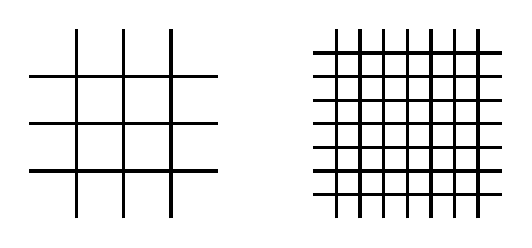
\begin{tikzpicture}[scale=1.2, very thick]
%the first one of these squares wasn't actually a 4-regular subdivision,
%since its only face had 2 sides instead of 4
%\Square{-3}{0}
\Square{0}{0}
\Square{3}{0}
%\draw (-3,-1) to (-3,1);
%\draw (-4,0) to (-2,0);

\foreach \x in {-0.5,0,0.5}
{
\draw (\x, -1) to (\x, 1);
\draw (-1, \x) to (1, \x);
}

\foreach \x in {-0.75,-0.5, ..., 0.75}
{
\draw (3+\x, -1) to (3+\x, 1);
\draw (2, \x) to (4, \x);
}
\end{tikzpicture}
\]
Obviously, in this way one can produce an infinite number of these examples on the torus.

The existence of an $n$-regular subdivision imposes strong conditions on the surface. In fact, suppose we have an $n$-regular subdivision of a surface and let $v, e$ and $f$ denote its number of vertices, edges and faces respectively. Since every face contains exactly $n$ vertices and every vertex belongs to exactly $n$ faces, we have that $v=f$. Moreover, every face contains $n$ edges and any edge belongs to exactly 2 faces, so $e=nf/2$.
Recalling the fact that the Euler characteristic of a surface of genus $g$ is $2-2g$, we have that $2-2g=v-e+f=(2-n/2)f$, or equivalently $4g-4 = (n-4)f$. If $n=4$, the right hand vanishes, and so $g=1$. Therefore, the only surface that can admit a $4$-regular subdivision is the torus (and in fact we have already shown there are an infinite number of them).

Suppose now that $n\neq 4$. Then
\begin{equation}
\label{euler-regular}f=\frac{4g-4}{n-4},
\end{equation}and so $g$ must be such that this quotient is integral. Moreover, since $n$ faces meet at every vertex, there must be at the very least $n$ faces, and so $n(n-4)\leq 4(g-1)$. Therefore, we have that $g\in \Omega(n^2)$.\note{no se si vale la pena observar esto}

All of these are \emph{necessary} conditions for an $n$-regular subdivision to exist. We have already shown an infinite number of examples of these objects, but we do not know if these subdivisions exist for any genus (or even for arbitrarily high genera).

\begin{exmp} Consider the complete graph $K_8$ with vertex set $\{1,2,\dots,8\}$. One may glue eight heptagons having the rows of the following matrix as edges:
\begin{center}
\begin{tabular}{ c  c  c  c  c  c  c }
1 &  2 &  3 &  4 &  5 &  6 &  7\\
2 &  1 &  3 &  7 &  5 &  8 &  6\\
3 &  2 &  4 &  1 &  6 &  8 &  7\\
4 &  3 &  5 &  2 &  7 &  8 &  1\\
5 &  4 &  6 &  3 &  1 &  8 &  2\\
6 &  5 &  7 &  4 &  2 &  8 &  3\\
7 &  6 &  1 &  5 &  3 &  8 &  4\\
1 &  7 &  2 &  6 &  4 &  8 &  5
\end{tabular}
\end{center}
In this way, we obtain an orientable, closed surface of genus seven, such that exactly seven heptagonal faces meet at every vertex; in other words, a 7-regular surface.
\end{exmp}

Our main interest in the concept of $n$-regularity lies in the following fact:

\begin{thm} The Jacobian algebra associated to an $n$-regular subdivision of a surface is infinite-dimensional.
\end{thm}
\begin{proof} We will first prove the case where $n>3$. Let $(Q,P)$ be the quiver with potential associated to the subdivision, $I$ the ideal in $\kQ$ spanned by the cyclic derivatives of the potential $P$ and $J$ the closure of $I$ in $\KQ$. 

Any arrow $x$ in the quiver is a factor of exactly two cycles in $P$: one of them is contained in the same face of the subdivision as $x$ and the other surrounds a vertex and is composed of arrows lying in different faces. The condition of $n$-regularity forces these two cycles to be of length $n$, and so $\partial_x(P)= a+b$, with $a$ and $b$ paths of length $n-1$. Therefore, $I$ is an homogeneous ideal, since it is spanned by homogeneous elements, and so $\kQ/I$ inherits a grading from $\kQ$. In fact, we introduced the notion of $n$-regularity solely to force the ideal $I$ to be homogeneous.

\begin{figure}[h]
\[
\begin{tikzpicture}[scale=1]
\draw (-3,1) to (3,1);
\draw (-3, -1) to (3, -1);
\draw (-1, -3) to (-1, 3);
\draw (1, -3) to (1, 3);
\draw[very thick, ->] (0.9, 0.1) to (0, 0.9);
\draw[red, very thick, ->] (-0.1, 0.9) to (-0.9, 0);
\draw[red, very thick, ->] (-0.9, -0.1) to (0, -0.9);
\draw[red, very thick, ->] (0.1, -0.9) to (0.9, 0);
\draw[blue, very thick, ->] (0.1, 1.1) to (0.9, 2);
\draw[blue, very thick, ->] (1.1, 1.9) to (1.9, 1.1);
\draw[blue, very thick, ->] (1.9, 0.9) to (1.1, 0.1);
\end{tikzpicture}
\]
\begin{caption}{Any cyclic derivative of the potential $P$ associated to a 4-regular subdivision turns out to be of the form $\textcolor{red}{a} + \textcolor{blue}{b}$, with both $\textcolor{red}{a}$ and $\textcolor{blue}{b}$ of length 3.}
\end{caption}
\end{figure}

Since $I$ is homogeneous, the quotient $\kQ/I$ turns out to be $\bigoplus A_n/(I\cap A_n)$, where $A_n$ stands for the graded component of degree $n$. The completion is then carried out componentwise, so $\KQ/J$ is actually $\prod A_n/(I\cap A_n)$. We have a natural inclusion $i:\kQ/I\to \KQ/J$, which is obviously not the case if the ideal is non-homogeneous, as one can infer from \hyperref[counterexample]{Example \ref*{counterexample}}. In the light of this fact, it suffices to show that $\kQ/I$ is infinite-dimensional.

The path algebra $\kQ$, regarded as a $k$-vector space, admits a direct sum decomposition $A\oplus B$, where $A$ is the subspace spanned by paths 
\[
\claim{containing either $n-1$ consecutive arrows belonging to the same face or $n-1$ consecutive arrows surrounding the same vertex of the subdivision as factors}\tag{$\clubsuit$}
\]
and $B$ is the subspace spanned by paths not satisfying $(\clubsuit)$. One immediately checks that $A$ is actually an ideal in $\kQ$. Even more, since every cyclic derivative is the sum of two paths satisfying $(\clubsuit)$, we have that $I\subseteq A$. Therefore, any non-zero path $c\in B$ is not contained in $I$, and in turn is not zero in $\kQ/I$.

Suppose now that $X$ is an infinite subset of $B$ composed of non-zero paths, all of different lengths. Since paths are homogeneous elements of $\kQ$ and $I$ is an homogeneous ideal, the projection of a path into $\kQ/I$ is an homogeneous element too. Therefore, the projection of $X$ into $\kQ/I$ is an infinite linearly independent set, since it is composed of non-zero homogeneous elements, each belonging to a different homogeneous component. So finally, all that remains to show is that one can actually produce such a set $X$.

Choose any path of length 2 contained in a single face and name it $x_2$. One may concatenate any path with exactly two arrows: one which lies on the same face as the last one and one which does not. If the two last arrows of $x_k$ lie on the same face, let $x_{k+1}$ be the path obtained from $x_k$ by concatenating the arrow lying on a different face. Otherwise, let $x_{k+1}$ be the path obtained from $x_k$ by concatenating the arrow lying on the same face as $x_k$'s last arrow. Since this process may be carried out indefinitely, we obtain a sequence $X=(x_k)_{k\geq 2}$ of paths, all of them of different lengths. Notice that every path $x_k$ is contained in $B$, since by construction it contains at most 2 consecutive arrows on the same face or around the same vertex, and $n-1 > 2$ by hypothesis. In fact, this construction can not be carried out if $n=3$, since in that case $B$ is the $k$-vector space spanned by paths of length $0$ and $1$.

This settles the case $n>3$ and now we turn to the study of the case $n=3$. By \hyperref[euler-regular]{Equation (\ref*{euler-regular})}, we know that $f=(4g-4)/(3-4)= 4-4g$. Since the number of faces in the subdivision must be positive, it follows that $g=0$, and so a 3-regular division of a surface must necessarily be a triangulation of a sphere consisting of 4 faces, or in other words a tetrahedron. We have already determined that the Jacobian algebra associated to the tetrahedron is infinite-dimensional in \hyperref[tetra]{Section \ref*{tetra}}, and so the proof is now complete.
\end{proof}
\end{section}

\begin{section}{A family of finite-dimensional examples}
We now turn to the study of another family of polygonal subdivisions, this time inducing finite-dimensional algebras. Let us start by showing that closed surfaces of any genus admit a particular decomposition.

A \emph{loop} $f$ on a surface $\Sigma$ is a smooth embedding $f:S^1\to \Sigma$. We will identify a loop with its image on $\Sigma$. A \emph{handle} is a torus with a disk removed. We recall that, by the classification theorem, a closed surface of genus $g>0$ can be obtained starting with a disk with $g-1$ holes and gluing handles along each hole and the boundary of the disk. 

\begin{figure}[h]
\centering
	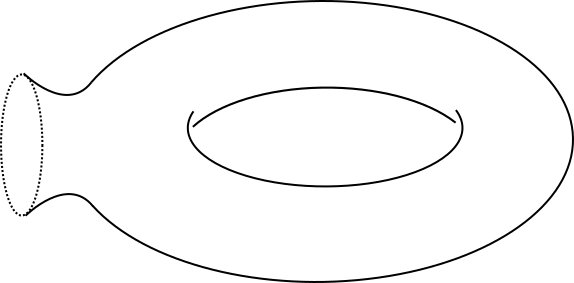
\includegraphics[width=0.5\textwidth]{handle.png}
\caption{A handle.}
\end{figure}

\begin{prop}\label{surface-loops} Let $\Sigma$ be a closed surface of genus $g$. There exist finite families $R=\{r_i\}$ and $B=\{b_j\}$ of loops on $\Sigma$ such that:
\begin{enumerate}
\item Two loops in the same family are disjoint.
\item Any point of the surface belongs to at most two loops.
\item The loops divide the surface into a disjoint family of regions, each of them a disk (up to homeomorphism).
\end{enumerate}
\end{prop}

\begin{proof} We give an explicit construction of such families.

The case in which $g=0$ (the sphere) is easily dealt with by choosing a single loop $r_1$ as the equator, since both hemispheres are homeomorphic to a disk and the other conditions are vacuously true.

For the cases in which $g>0$, we will make use of the handle decomposition we mentioned previously. We will draw a handle as a square (with opposite edges identified) having a gray hole in its center. Consider the following configuration:

\begin{figure}[h]
\label{divided-handle}
\[
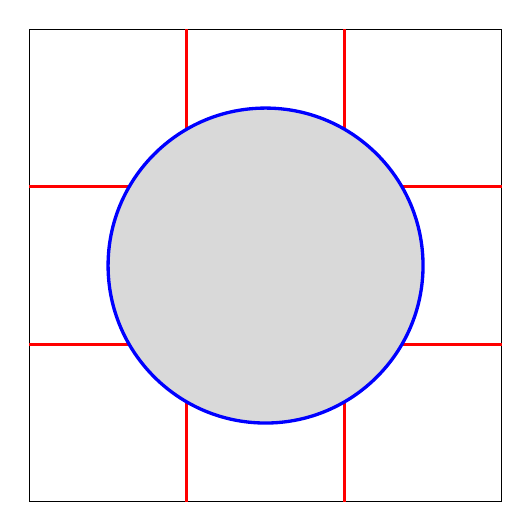
\begin{tikzpicture}
\draw (0,0) node[minimum size=6cm,draw] {};

\fill [black,opacity=.15] circle (2cm);

\draw[red, very thick] (-3,1) -- (-1.73,1);
\draw[red, very thick] (-3,-1) -- (-1.73,-1);

\draw[red, very thick] (3,1) -- (1.73,1);
\draw[red, very thick] (3,-1) -- (1.73,-1);

\draw[red, very thick] (1,-3) -- (1,-1.73);
\draw[red, very thick] (-1,-3) -- (-1,-1.73);

\draw[red, very thick] (1,3) -- (1,1.73);
\draw[red, very thick] (-1,3) -- (-1,1.73);

\draw[blue, very thick] (0,0) circle (2cm);
\end{tikzpicture}
\]
\caption{}
\end{figure}

We first deal with the case in which $g=1$. If we glue such a handle to the boundary of the following disk, we obtain a torus with a single red loop $r_1$ and a single blue loop $b_1$:

\begin{figure}[h]
\[
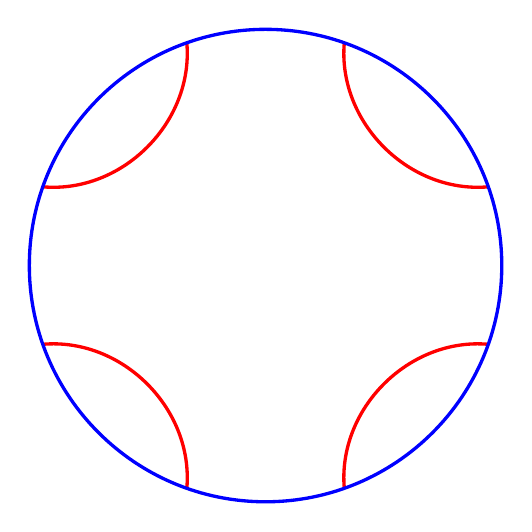
\begin{tikzpicture}

\draw[red, very thick] (-2.83,1) to [bend right=50] (-1,2.83);
\draw[red, very thick] (2.83,1) to [bend left=50] (1,2.83);
\draw[red, very thick] (2.83,-1) to [bend right=50] (1,-2.83);
\draw[red, very thick] (-2.83,-1) to [bend left=50] (-1,-2.83);

\draw[blue, very thick] (0,0) circle (3cm);
\end{tikzpicture}
\]
\end{figure}

Once again, the intersection conditions are vacuous. Finally, we observe that the blue loop cuts the torus into a disk and a handle, so one can check condition $3$ in both objects separately. One sees at once that the disk gets cut up into 5 smaller disks, while the handle is divided into $3$ disks, as we wanted.

While the solution to the case $g=1$ may be easier to draw directly on a square instead of considering a handle decomposition, the latter helps to illustrate the general case, which we now consider. For the case $g>1$, we regard our surface as a disk with $g-1$ holes, with a handle divided as in \hyperref[divided-handle]{Figure \ref*{divided-handle}} attached to its boundary and to each of its holes. We now exemplify the configuration on the disk with holes for $g=4$:

\begin{figure}[h]
\[
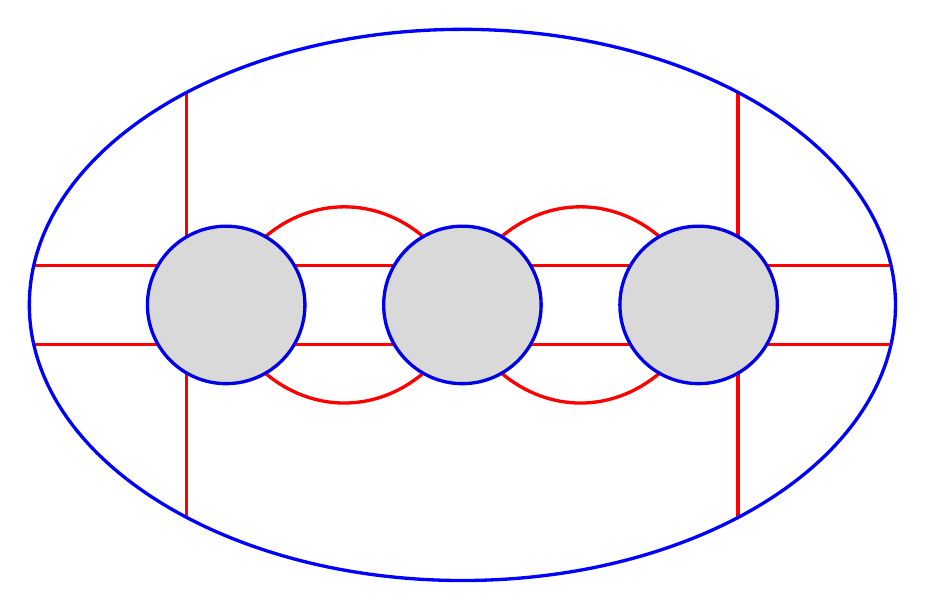
\begin{tikzpicture}
\draw[red, very thick] (-5.44, 0.5) -- (-3.87, 0.5);
\draw[red, very thick] (-5.44, -0.5) -- (-3.87, -0.5);
\draw[red, very thick] (5.44, 0.5) -- (3.87, 0.5);
\draw[red, very thick] (5.44, -0.5) -- (3.87, -0.5);

\draw[red, very thick] (-3.5,0.87) -- (-3.5,2.7);
\draw[red, very thick] (-3.5,-0.87) -- (-3.5,-2.7);
\draw[red, very thick] (3.5,0.87) -- (3.5,2.7);
\draw[red, very thick] (3.5,-0.87) -- (3.5,-2.7);

\draw[red, very thick] (-2.137, 0.5) -- (-0.863, 0.5);
\draw[red, very thick] (-2.137, -0.5) -- (-0.863, -0.5);
\draw[red, very thick] (2.137, 0.5) -- (0.863, 0.5);
\draw[red, very thick] (2.137, -0.5) -- (0.863, -0.5);

\draw[red, very thick] (-2.5,0.87) to [bend left=40] (-0.5,0.87);
\draw[red, very thick] (2.5,0.87) to [bend right=40] (0.5,0.87);
\draw[red, very thick] (-2.5,-0.87) to [bend right=40] (-0.5,-0.87);
\draw[red, very thick] (2.5,-0.87) to [bend left=40] (0.5,-0.87);

\draw[blue, very thick] (0,0) ellipse (5.5cm and 3.5cm);
\draw[blue, very thick] (0,0) circle (1cm);
\draw[blue, very thick] (-3,0) circle (1cm);
\draw[blue, very thick] (3,0) circle (1cm);
\fill [black,opacity=.15] (-3,0) circle (1cm);
\fill [black,opacity=.15] (0,0) circle (1cm);
\fill [black,opacity=.15] (3,0) circle (1cm);
\end{tikzpicture}
\]
\end{figure}

The following is an outline for the construction of the previous figure for general $g$:
\begin{enumerate}
\item Place the $g-1$ holes in a straight line inside the disk.
\item Connect the boundary of the left and rightmost holes to the boundary of the disk using 4 red arcs, mimicking the figure.
\item Cycle through the holes from left to right. If the current hole has a neighboring hole to its right, draw 4 red arcs connecting their boundaries.
\end{enumerate}

Notice that after gluing the handles, both the red and the blue arcs are now loops. We now consider the families $\{r_i\}$ and $\{b_j\}$, consisting of the red and blue loops respectively. Inspecting the figures, we see that conditions 1 and 2 are both satisfied. Finally, it remains to check condition 3. Since we have already seen that each handle is split up into disks in the discussion of the case $g=1$, it suffices to check this for the disk with holes, and once again this is easily seen in the drawing.
\end{proof}

A \emph{band} on a surface $\Sigma$ is a finite sequence $\{C_1, \dots, C_n\}$, where each $S_i$ is a square on $\Sigma$ subdivided by one of its main diagonals, arranged as in one of the following two figures:
\[
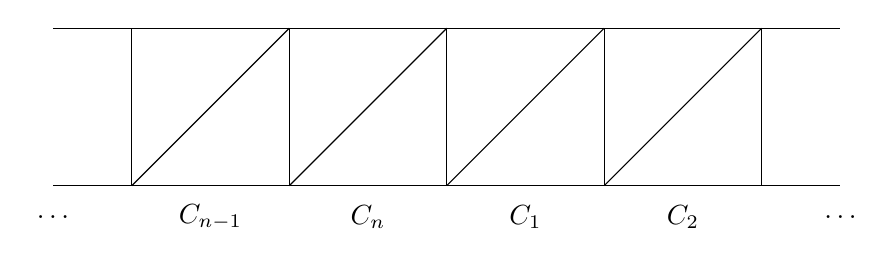
\begin{tikzpicture}
\draw (-5,1) -- (5,1);
\draw (-5,-1) -- (5,-1);

\foreach \x in {-4,-2,...,4}
\draw (\x,1) -- (\x,-1);

\foreach \x in {-4,-2,...,2}
\draw (\x,-1) -- (\x+2, 1);

\node at (-5,-1.4) {$\dots$};
\node at (-3,-1.4) {$C_{n-1}$};
\node at (-1,-1.4) {$C_{n}$};
\node at (1,-1.4) {$C_{1}$};
\node at (3,-1.4) {$C_{2}$};
\node at (5,-1.4) {$\dots$};
\end{tikzpicture}
\]
\[
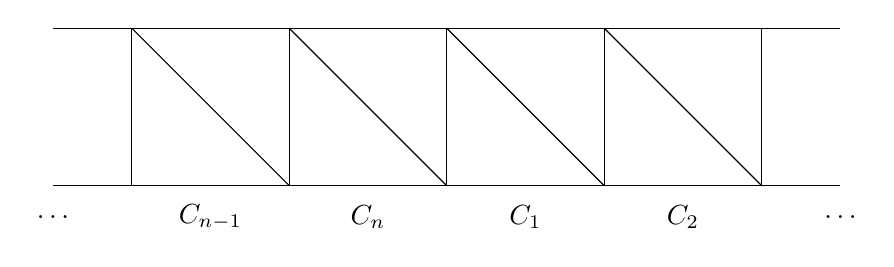
\begin{tikzpicture}
\draw (-5,1) -- (5,1);
\draw (-5,-1) -- (5,-1);

\foreach \x in {-4,-2,...,4}
\draw (\x,1) -- (\x,-1);

\foreach \x in {-4,-2,...,2}
\draw (\x,1) -- (\x+2, -1);

\node at (-5,-1.4) {$\dots$};
\node at (-3,-1.4) {$C_{n-1}$};
\node at (-1,-1.4) {$C_{n}$};
\node at (1,-1.4) {$C_{1}$};
\node at (3,-1.4) {$C_{2}$};
\node at (5,-1.4) {$\dots$};
\end{tikzpicture}
\]

Notice that in both cases the choice of diagonal is consistent throughout the band. We will say a band is \emph{positively oriented} if it is arranged as in the first figure and \emph{negatively oriented} otherwise (we stress that this makes sense since the surface is oriented). We require that the only adjacency relations between squares in a band are the ones expressed by the figures, so in particular bands have well-defined top and bottom sides. We remark that two differently oriented bands may intersect as the following figure shows: 

\begin{figure}[h]
\centering
\begin{tikzpicture}[scale=.65]
\foreach \x in {-4,-2,...,4}
{
\DSquare{\x}{0}
\DSquare{0}{\x}
}
\draw (-1, -6) to (-1, -5);
\draw (1, -6) to (1, -5);
\draw (-1, 6) to (-1, 5);
\draw (1, 6) to (1, 5);
\draw (-6,-1) to (-5,-1);
\draw (-6,1) to (-5,1);
\draw (6,-1) to (5,-1);
\draw (6,1) to (5,1);
\end{tikzpicture}
\caption{Two intersecting bands.}
\label{band-intersection}
\end{figure}

Given a surface $\Sigma$ of arbitrary genus, we consider families of loops $R=\{r_i\}$ and $B=\{b_j\}$ on $\Sigma$ satisfying the conditions stated in \hyperref[surface-loops]{Proposition \ref*{surface-loops}}. We can now pick suitably small tubular neighborhoods of each loop and place a positively (resp. negatively) oriented band over each neighborhood corresponding to a loop in $R$ (resp. $B$). Conditions 1 and 2 of \hyperref[surface-loops]{Proposition \ref*{surface-loops}} guarantee that all intersections between bands resemble that of \hyperref[band-intersection]{Figure \ref*{band-intersection}}. Condition 3 guarantees that each connected component of the complement of the bands is a polygon. We will refer to these polygons as \emph{regions}. Therefore, the collection of bands and regions actually define a polygonal subdivision of $\Sigma$. For technical reasons that will be clearer later, we will require each band to
\[
\label{diamondhyp}
\claim{have at least 5 squares between any pair of intersections with other bands.}\tag{$\diamond$}
\]
This can be easily achieved by refining the division of the band if necessary. From now on we fix a subdivision as described above for each genus $g$ and call its associated QP $(Q_g,P_g)$. The corresponding Jacobian algebra will be denoted $A_g$.

\begin{figure}[h]
\[
\begin{tikzpicture}[scale=0.7]
\foreach \x in {-6,-4,...,6}
{
\ArrowedSquare{\x}{6}
\ArrowedSquare{\x}{-6}
\ArrowedSquare{6}{\x}
\ArrowedSquare{-6}{\x}
}
\draw (-8,-7) to (-7,-7);
\draw (-8,-5) to (-7,-5);
\draw (8,-7) to (7,-7);
\draw (8,-5) to (7,-5);
\draw (-8,7) to (-7,7);
\draw (-8,5) to (-7,5);
\draw (8,7) to (7,7);
\draw (8,5) to (7,5);
\draw (-7,-8) to (-7,-7);
\draw (-5,-8) to (-5,-7);
\draw (-7,8) to (-7,7);
\draw (-5,8) to (-5,7);
\draw (7,-8) to (7,-7);
\draw (5,-8) to (5,-7);
\draw (7,8) to (7,7);
\draw (5,8) to (5,7);
\foreach \x in {-4,-2,...,2}
{
\draw[<-, red, very thick] (-6+1.1, \x + 0.1) to [bend right] (-6+1.1, \x + 1.9);
\draw[->, red, very thick] (6-1.1, \x + 0.1) to [bend left] (6-1.1, \x + 1.9);
\draw[->, red, very thick] (\x + 0.1,-6+1.1) to [bend left] (\x + 1.9,-6+1.1);
\draw[<-, red, very thick] (\x + 0.1, 6-1.1) to [bend right] (\x + 1.9, 6-1.1);
}
\draw[->, red, very thick] (-4-0.1, 6-1.1) to [bend left] (-6+1.1, 4+0.1);
\draw[<-, red, very thick] (4+0.1, 6-1.1) to [bend right] (6-1.1, 4+0.1);
\draw[<-, red, very thick] (6-1.1, -4-0.1) to [bend right] (4+0.1, -6+1.1);
\draw[->, red, very thick] (-6+1.1, -4-0.1) to [bend left] (-4-0.1,-6+1.1);
\end{tikzpicture}
\]
\caption{The configuration of the associated quiver $Q_g$ around a region satisfying \hyperref[diamondhyp]{$(\diamond)$}.}
\end{figure}
We now turn to the study of some relations that hold in $A_g$, that will enable us to prove its finite-dimensionality.

\begin{lemma}\label{band-sides} Any path in $A_g$ passing through vertices of both sides of a band is zero.
\end{lemma}
\begin{proof} Throughout this and the following proofs, we will only consider our bands to be positively oriented, since the analogous statements for negatively oriented bands are proved in a similar fashion. We name the arrows in the quiver as in the following figure:
\[
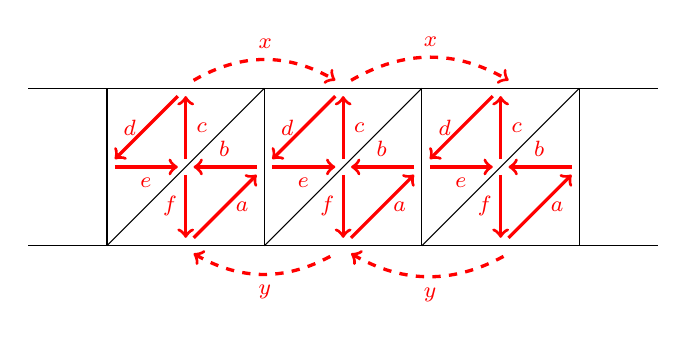
\begin{tikzpicture}[text width=1.5mm, font=\footnotesize]
\draw (-4, 0) -- (4, 0);
\draw (-4, 2) -- (4, 2);
\foreach \x in {-3,-1,...,3}
\draw (\x, 0) -- (\x, 2);
\foreach \x in {-3,-1,1}
{
\draw (\x,0) -- (\x+2, 2);
\draw [->, red, very thick] (\x+1.9, 1) to node[above] {$b$} (\x+1.1, 1);
\draw[->, red, very thick] (\x+1, 0.9) to node[left]{$f$} (\x+1, 0.1);
\draw[->, red, very thick] (\x+1.1, 0.1) to node[right]{$a$} (\x+1.9, 0.9);
\draw[->, red, very thick] (\x+1, 1.1) to node[right]{$c$} (\x+1, 1.9);
\draw[->, red, very thick] (\x+0.9, 1.9) to node[left]{$d$} (\x+0.1, 1.1);
\draw[->, red, very thick] (\x+0.1, 1) to node[below]{$e$} (\x+0.9, 1);
}

\draw[->, red, dashed, very thick] (-1.9, 2.1) to [bend left] node[above]{$x$} (-0.1, 2.1);
\draw[->, red, dashed, very thick] (0.1, 2.1) to [bend left] node[above]{$x$} (2.1, 2.1);
\draw[<-, red, dashed, very thick] (-1.9, -0.1) to [bend right] node[below]{$y$} (-0.1, -0.1);
\draw[<-, red, dashed, very thick] (0.1, -0.1) to [bend right] node[below]{$y$} (2.1, -0.1);
\end{tikzpicture}
\]

Since our quiver arises from a polygonal subdivision of a surface with \emph{empty} boundary, we know that there is a cycle around each vertex, and so each $x$ and each $y$ are paths of length at least 1. We mark those paths in the figure with a dashed arrow. We have given the same name to arrows occupying the same position in different squares, since this abuse of notation will be useful for calculation.

Inspecting the figure we see that any path passing through vertices of both sides of the band must contain a path of the form $cba$ or $fed$ as factors. It suffices to check that both of them are zero in $A_g$.

We have that $\partial_f(P_g) = ba + eay$, and so $ba  = -eay$ in $A_g$. Therefore, we have that $cba = -ceay$. Moreover, $\partial_d(P_g) = ce + xcb$, from which we deduce that $ce = -xcb$ in $A_g$. Putting all of this together, we get that $cba=-ceay=xcbay$ (one should note that the $cba$ factor in the right hand side of the equality consists of arrows placed on the square immediately left from the one where we started). Proceeding inductively we get $cba=x^ncbay^n$ for all positive $n$. Since $x$ and $y$ are paths of length at least $1$, this shows that $cba$ is equal to paths of arbitrarily high length. Therefore, by \hyperref[arbitrarily-long]{Observation \ref*{arbitrarily-long}}, we conclude that $cba=0$ in $A_g$.

An analogous argument shows that $fed=0$ in $A_g$ as well, concluding the proof. 
\end{proof}

\begin{lemma}\label{long-band-paths} Any sufficiently long path contained entirely in bands is zero in $A_g$. More precisely, any non-zero path contained in a single band (resp. several bands) is of length at most 5 (resp. 9).
\end{lemma}
\begin{proof} We first prove that any sufficiently long path contained entirely in a single band is zero. As we have already seen, any path passing through vertices of both sides of the band is zero, so we will suppose without loss of generality that our path is placed on the upper part of the band. Maintaining the notation used on the proof of the previous lemma, this is equivalent to saying our path only has arrows $b, c, d$ or $e$ as factors.

We start by studying paths containing a $3$-cycle as a prefix. The $3$-cycles $edc$ and $ced$ only prefix two paths of length 4, namely $cedc$ and $dced$. Since $\partial_e(P_g) = dc + ayf$, the relation $dc = -ayf$ holds, and so $cedc=-ceayf=0$ and $dced=-ayfed=0$ by \hyperref[band-sides]{Lemma \ref*{band-sides}}. Moreover, the $3$-cycle $dce$ only prefixes two paths of length 5, which are $cbdce$ and $cedce$. Clearly, $cedce=0$ since we have already shown that $cedc=0$, and using the relation $dc=-ayf$ we get $cbdce = - cbayfe=0$ once again by \hyperref[band-sides]{Lemma \ref*{band-sides}}.

Now we turn to paths containing a $3$-cycle as a suffix. Once again, the $3$-cycles $ced$ and $dce$ only suffix two paths of length 4, which are $cedc$ and $dced$, already shown to be zero. The $3$-cycle $edc$ is a suffix to only two paths of length 5, which are $edcbd$ and $edced$. We see that $edced=0$ since $dced=0$ and $edcbd=-eayfbd=0$ as we wanted.

Therefore, any path in a band of length greater than 5 containing a 3-cycle is zero, since we have shown these cycles only admit prefixes and suffixes of length at most 1.

Now, a path of length greater than 5 not containing a 3-cycle is either of the form $dcbdcb$, $bdcbdc$ or $cdbcbd$. All possibilites have $cbdc$ as a factor, which is clearly zero since $cbdc = -cbayf = 0$ by \hyperref[band-sides]{Lemma \ref*{band-sides}}. Therefore, we conclude that any path of length greater than 5 contained in a single band is zero.

Finally, consider a path of length greater than 9 contained in possibly different bands. If its first six arrows lie on the same band, the path is zero as seen previously. Otherwise, at most five of its first arrows lie on the same band and the sixth is then placed on a different band intersecting the original one, as seen in the following figure:
\[
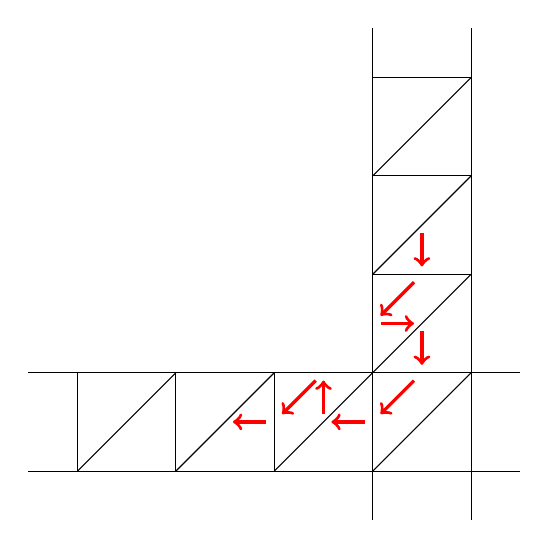
\begin{tikzpicture}
\draw (-3.5*1.25, 0) -- (1.5*1.25, 0);
\draw (-3.5*1.25, -1.25) -- (1.5*1.25, -1.25);
\draw (0,3.5*1.25) -- (0,-1.5*1.25);
\draw (1.25,3.5*1.25) -- (1.25,-1.5*1.25);

\foreach \x in {-3.75,-2.5,...,0}
{
\draw (\x,-1.25) -- (\x+1.25, 0);
\draw (0, -\x) -- (1.25, -\x);
\draw (\x,0) -- (\x, -1.25);
}

\foreach \x in {0,1.25,...,2.5}
\draw (0, \x) -- (1.25, \x+1.25);

\draw[->, red, very thick] (0.5*1.25, 1.5*1.25 - 0.1) -- (0.5*1.25, 1.25 + 0.1);
\draw[->, red, very thick] (0.5*1.25 - 0.1, 1.25-0.1) -- (0.1, 0.5*1.25+0.1);
\draw[->, red, very thick] (0.1, 0.5*1.25) -- (0.5*1.25 - 0.1, 0.5*1.25);
\draw[->, red, very thick] (0.5*1.25, 0.5*1.25-0.1) -- (0.5*1.25, 0.1);
\draw[->, red, very thick] (0.5*1.25 - 0.1, -0.1) -- (0.1, -0.5*1.25+0.1);
\draw[->, red, very thick] (-0.1, -0.5*1.25) -- (-0.5*1.25+0.1, -0.5*1.25);
\draw[->, red, very thick] (-0.5*1.25, -0.5*1.25+0.1) -- (-0.5*1.25, -0.1);
\draw[->, red, very thick] (-0.5*1.25 - 0.1, -0.1) -- (-1.25 + 0.1, -0.5*1.25+0.1);
\draw[->, red, very thick] (-1.25 -0.1, -0.5*1.25) -- (-1.5*1.25+0.1, -0.5*1.25);
\end{tikzpicture}
\]

Since by hypothesis \hyperref[diamondhyp]{$(\diamond)$} two intersections in the same band are distanced by at least five squares, we conclude that at least the next six arrows belong to the same band. Therefore, any path of length greater than 9 contained entirely in bands is zero in $A_g$, as we wanted.
\end{proof}

\begin{lemma}\label{long-region-paths} Any non-zero path entirely contained in an $n$-sided region is of length at most $3n-4$.
\end{lemma}
\begin{proof} We fix an $n$-sided region. Consider any band neighboring our region and pick any of its squares that is at least two squares away from an intersection with another band, which is always possible by hypothesis \hyperref[diamondhyp]{$(\diamond)$}. Recalling the fact that our region induces an $n$-cycle in the quiver, we name the arrow starting at the square we picked as $x_0$. In general, given $j\in \ZZ/n\ZZ$ we call $x_j$ the arrow starting at the target of $x_{j-1}$. Keeping the previous notation for arrows contained in bands, our current situation is illustrated by this figure:
\[
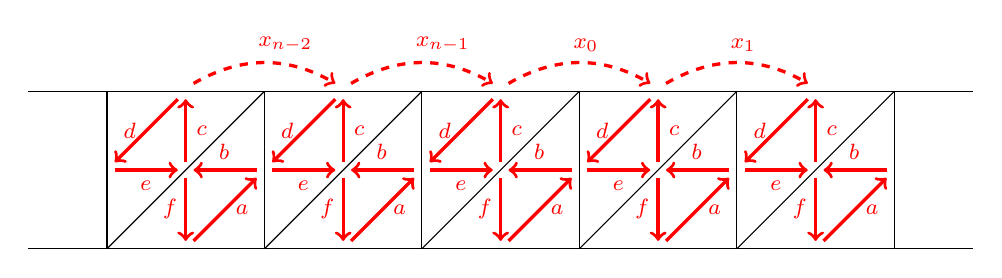
\begin{tikzpicture}[text width=1.5mm, font=\footnotesize]
\draw (-6, 0) -- (6, 0);
\draw (-6, 2) -- (6, 2);
\foreach \x in {-5,-3,...,5}
\draw (\x, 0) -- (\x, 2);
\foreach \x in {-5,-3,...,3}
{
\draw (\x,0) -- (\x+2, 2);
\draw [->, red, very thick] (\x+1.9, 1) to node[above] {$b$} (\x+1.1, 1);
\draw[->, red, very thick] (\x+1, 0.9) to node[left]{$f$} (\x+1, 0.1);
\draw[->, red, very thick] (\x+1.1, 0.1) to node[right]{$a$} (\x+1.9, 0.9);
\draw[->, red, very thick] (\x+1, 1.1) to node[right]{$c$} (\x+1, 1.9);
\draw[->, red, very thick] (\x+0.9, 1.9) to node[left]{$d$} (\x+0.1, 1.1);
\draw[->, red, very thick] (\x+0.1, 1) to node[below]{$e$} (\x+0.9, 1);
}

\draw[->, red, dashed, very thick] (-5+1.1, 2.1) to [bend left] node[above]{$\mathclap{x_{n-2}}$} (-5+2.9, 2.1);
\draw[->, red, dashed, very thick] (-3+1.1, 2.1) to [bend left] node[above]{$\mathclap{x_{n-1}}$} (-3+2.9, 2.1);
\draw[->, red, dashed, very thick] (-1+1.1, 2.1) to [bend left] node[above]{$\mathclap{x_{0}}$} (-1+2.9, 2.1);
\draw[->, red, dashed, very thick] (1+1.1, 2.1) to [bend left] node[above]{$\mathclap{x_{1}}$} (1+2.9, 2.1);
\end{tikzpicture}
\]

We now prove that the path $L=x_{n-1}x_{n-2}\dots x_2x_1x_{0}x_{n-1}\dots x_3x_2$ is zero. We have that $\partial_{x_0}(P_g)=x_{n-1}x_{n-2}\dots x_2x_1+cbd$ and $\partial_{x_1}(P_g)=x_{0}x_{n-1}\dots x_3x_2+cbd$. Therefore, the relations
\begin{align*}
x_{n-1}x_{n-2}\dots x_2x_1=-cbd\\
x_{0}x_{n-1}\dots x_3x_2=-cbd
\end{align*}
hold in $A_g$. We stress that $cbd$ denotes a different path in each one of the two equations: they are similar paths contained in different squares. Using these relations, we see that $$x_{n-1}x_{n-2}\dots x_2x_1x_{0}x_{n-1}\dots x_3x_2=-cbdx_{0}x_{n-1}\dots x_3x_2=cbdcbd,$$ and the latter is zero by \hyperref[long-band-paths]{Lemma \ref*{long-band-paths}} since $cbdcbd$ is a path of length 6 lying on a single band. 

Finally, since the longest path entirely contained in our region not having $L$ as a factor is
\[\underbrace{x_{n-2}x_{n-1}\dots x_0}_{\text{$n-1$ arrows}}\underbrace{x_{n-1}x_{n-2}\dots x_0}_{\text{$n$ arrows}}\underbrace{x_{n-1}x_{n-2}\dots x_3}_{\text{$n-3$ arrows}},\]
which is of length $3n-4$, the result follows.
\end{proof}

\begin{lemma} \label{long-br-paths} Any sufficiently long path not having factors from two different regions is zero in $A_g$.
\end{lemma}
\begin{proof} We write our path as $B_{k+1}R_k\dots R_2 B_2 R_1 B_1$, where the paths $R_i$ are contained in a same region and the paths $B_j$ are non-trivial (except possibly for $B_1$ and $B_{k+1}$) and contained in bands.

Let $1<j<k+1$. The path $B_j$ starts and ends at the boundary of our region of interest. Therefore, it must pass through both of the endpoints of a same arrow, which we will call $x_0$, belonging to the cycle associated to the region, since otherwise it would be sufficiently long as to reduce to zero, by \hyperref[long-band-paths]{Lemma \ref*{long-band-paths}}. Using the relation induced by $\partial_{x_0}(P_g)$, we can replace some of the arrows in $B_j$ with a path entirely contained in the region.
After applying this argument repeatedly, we can then suppose our path is of the form $B_2 R_1 B_1$. The proof now follows from \hyperref[long-band-paths]{Lemmas \ref*{long-band-paths}} and \ref{long-region-paths}, since if our path is non-zero, then $|B_1|<10$, $|B_2|<10$ and $|R_1|<3n-3$, where $n$ is the number of sides of the region.
\end{proof}

After proving all these lemmas, the main result of this section now follows easily:

\begin{thm} The algebra $A_g$ is finite-dimensional.
\end{thm}
\begin{proof} By \hyperref[long-br-paths]{Lemma \ref*{long-br-paths}}, any sufficiently long path is zero if it does not have factors from two different regions, but any path that does must be zero (regardless of length) by \hyperref[band-sides]{Lemma \ref*{band-sides}}, since it must cross a band. Since any sufficiently long path is zero, we conclude that $A_g$ is finite-dimensional.
\end{proof}
\end{section}

\begin{section}{Pyramids}
\label{pyramids}
A \emph{pyramid} is a polyhedron formed by placing a regular polygon (called the \emph{base}) and a single point (called the \emph{apex}) in different parallel planes, and then taking their convex hull. One immediately checks that if the base is an $n$-sided polygon, then the pyramid has exactly $n+1$ faces, $n$ of them triangles and the last one being the base itself.
Any pyramid is a polygonal subdivision of the sphere, so we now study the properties of its associated Jacobian algebra. We first label the arrows in the associated quiver as shown in 
\hyperref[pyramid-quiver]{Figure \ref*{pyramid-quiver}}.

\begin{figure}[h]
\label{pyramid-quiver}
\[
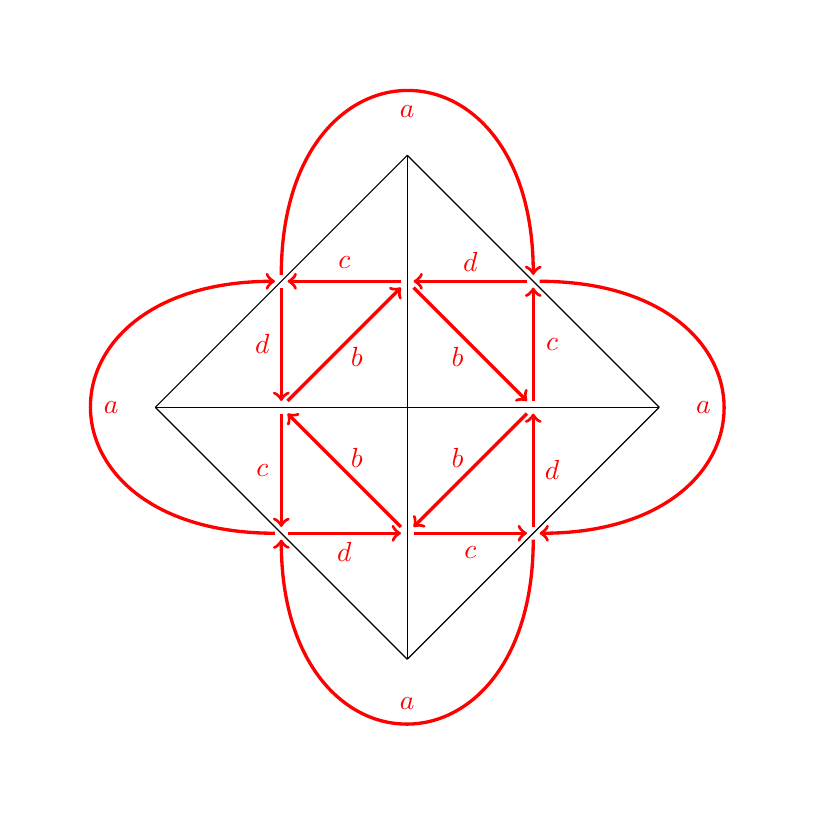
\begin{tikzpicture}[scale=0.8]
\foreach \x in {0,90,...,270}
{
\begin{scope}[rotate=\x]
\draw (0,0) -- (4,0);
\draw (0,0) -- (0,-4);
\draw (4,0) -- (0,-4);
\node at (0.8,-0.8) {\textcolor{red}{$b$}};
\node at (1,-2.3) {\textcolor{red}{$c$}};
\node at (2.3,-1) {\textcolor{red}{$d$}};
\node at (0,-4.7) {\textcolor{red}{$a$}};
\draw [<-, red, very thick] (0.1, -1.9) to (1.9, -0.1);
\draw [<-, red, very thick] (2, -0.1) to  (2, -1.9);
\draw [<-, red, very thick] (1.9, -2) to  (0.1, -2);
\draw [<-, red, very thick] (-2, -2.1) to [bend right=90, looseness=2.5] (2, -2.1);
\end{scope}
}
\end{tikzpicture}
\]
\caption{The quiver arising from a pyramid with a square base.}
\label{pyramid}
\end{figure}

The 4-cycle placed outside of the square is the cycle corresponding to the base, and each 3-cycle inside of the square corresponds to a triangular face of the pyramid. We will name the arrows of the base as $a$ and the arrows surrounding the apex as $b$. The rest of the arrows corresponding to triangular faces are named $c$ and $d$ in such a way that $dcb$ is the only path of length 3 taking place in a single triangle.

\begin{thm} Let $n\geq 3$. The Jacobian algebra associated to a pyramid with an $n$-sided base is finite-dimensional iff $n$ is even.
\end{thm}
\begin{proof} The case $n=3$ has already been covered in \hyperref[tetra]{Section \ref*{tetra}}, since a pyramid with a 3-sided base is just a tetrahedron. We will then suppose that $n> 3$.

We call $(Q,P)$ the QP associated to the pyramid and $A$ its Jacobian algebra. We will study $A$ making heavy use of the diamond lemma. To do so, we will order terms according first to length (longer terms being smaller) and then lexicographically from right to left. For instance, $a^5 \prec bd$ and $bda \prec b^3$. This is a minor modification of the usual revglex order (since words are sorted lexicographically but from right to left), and the same argument as in \hyperref[noeth-norm]{Lemma \ref*{noeth-norm}} proves that it satisfies the descending chain condition in norm.

The careful reader will note that, a priori, we are not under the hypotheses of the diamond lemma, since we have not specified a term order for the entire set of paths, but rather we have given an equivalence relation on the set of paths (where two paths are considered to be equal if they are given the same label) and then ordered the set of equivalence classes. This is of course no obstruction, since we may number the arrows carrying the same label and sort them first by their labels and then by their numbering. For instance, two different paths of the form $a^3$ may be numbered as, say, $a_2a_1a_0$ and $a_3a_2a_1$.

We now have to find a confluent reduction system compatible with our term order. We start off by computing the cyclic derivatives of the potential $P$, which turn out to be:
\begin{align*}
\partial_a(P) &= a^{n-1} + cd\\
\partial_b(P) &= b^{n-1} + dc\\
\partial_c(P) &= bd + da\\
\partial_d(P) &= ac + cb
\end{align*}
This suggests the following reduction system, which we will call $\Gamma$:
\begin{align*}
cd &\leadsto -a^{n-1}\tag{$\partial_a$}\\
dc &\leadsto -b^{n-1}\tag{$\partial_b$}\\
bd &\leadsto -da\tag{$\partial_c$}\\
ac &\leadsto -cb\tag{$\partial_d$}
\end{align*}
Every reduction rule is compatible with our term order, since the right hand side terms are either longer (since $n>3$) or of the same length but lexicographically smaller. Notice that the ideal $I_\Gamma$ generated by this reduction system is exactly the Jacobian ideal, so if the system turns out to be confluent, then the set of irreducible paths forms a basis for the Jacobian algebra $A$. The system $\Gamma$ presents only a few ambiguities, namely the ones arising from the monomials $cdc$, $dcd$, $bdc$ and $acd$. We now check if they are resolvable:
\[
\begin{tikzpicture}
\node (1) at (0,0) {$cdc$};
\node (a2) at (2,1) {$-a^{n-1}c$};
\node (b2) at (2,-1) {$-cb^{n-1}$};
\node (a3) at (7,1) {$(-1)^n cb^{n-1}$};
\draw[->] (1) to node[above, font=\footnotesize]{$\partial_a$} (a2);
\draw[->] (1) to node[below, font=\footnotesize]{$\partial_b$} (b2);
\draw[->] (a2) to node[above, font=\footnotesize]{$\partial_d$ ($n-1$ times)} (a3);
\end{tikzpicture}
\]
\[
\begin{tikzpicture}
\node (1) at (0,0) {$dcd$};
\node (a2) at (2,1) {$-b^{n-1}d$};
\node (b2) at (2,-1) {$-da^{n-1}$};
\node (a3) at (7,1) {$(-1)^n da^{n-1}$};
\draw[->] (1) to node[above, font=\footnotesize]{$\partial_b$} (a2);
\draw[->] (1) to node[below, font=\footnotesize]{$\partial_a$} (b2);
\draw[->] (a2) to node[above, font=\footnotesize]{$\partial_c$ ($n-1$ times)} (a3);
\end{tikzpicture}
\]
\[
\begin{tikzpicture}
\node (1) at (0,0) {$bdc$};
\node (a2) at (2,1) {$-dac$};
\node (b2) at (2,-1) {$-b^n$};
\node (a3) at (4,1) {$dcb$};
\node (a4) at (6,1) {$-b^n$};
\draw[->] (1) to node[above, font=\footnotesize]{$\partial_c$} (a2);
\draw[->] (1) to node[below, font=\footnotesize]{$\partial_b$} (b2);
\draw[->] (a2) to node[above, font=\footnotesize]{$\partial_d$} (a3);
\draw[->] (a3) to node[above, font=\footnotesize]{$\partial_b$} (a4);
\end{tikzpicture}
\]
\[
\begin{tikzpicture}
\node (1) at (0,0) {$acd$};
\node (a2) at (2,1) {$-cbd$};
\node (b2) at (2,-1) {$-a^n$};
\node (a3) at (4,1) {$cda$};
\node (a4) at (6,1) {$-a^n$};
\draw[->] (1) to node[above, font=\footnotesize]{$\partial_d$} (a2);
\draw[->] (1) to node[below, font=\footnotesize]{$\partial_a$} (b2);
\draw[->] (a2) to node[above, font=\footnotesize]{$\partial_c$} (a3);
\draw[->] (a3) to node[above, font=\footnotesize]{$\partial_a$} (a4);
\end{tikzpicture}
\]
As we can see, the rewriting system $\Gamma$ turns out to be confluent iff $n$ is odd, since our ground field $k$ is of characteristic zero. In that case, we know that the set of irreducible terms forms a basis of the Jacobian algebra. Since paths of the form $a^k$ and $b^k$ are irreducible for any $k$, we conclude that the Jacobian algebra is infinite-dimensional for odd values of $n$.

As for the even case, we may try to enlarge the set of rewriting rules as to make the system confluent. From our previous computation using our old rewriting system $\Gamma$, we know that $cb^{n-1}=da^{n-1}=0$. Moreover,  $0=dcb^{n-1}=-b^{2n-2}$ and  $0=cda^{n-1}=-a^{2n-2}$. We may consider the rewriting system $\Gamma'$, composed of the old set of rewriting rules from $\Gamma$ and the following new rules:
\begin{align*}
da^{n-1} &\leadsto 0 \\
cb^{n-1} &\leadsto 0\\
a^{2n-2} &\leadsto 0\\
b^{2n-2} &\leadsto 0
\end{align*}
We remark that this system is compatible with our term order. Moreover, the ideal $I_{\Gamma'}$ coincides with the Jacobian ideal as well, since the new rules come from identities holding in the Jacobian algebra $A$. It suffices to check that $\Gamma'$ is indeed a confluent system in order to be in the hypotheses of the diamond lemma. The set of ambiguities is now slightly larger: it contains all of the old ones (which are now resolvable, thanks to the rules $da^{n-1} \leadsto 0$ and $cb^{n-1} \leadsto 0$) plus the ambiguities arising from the following set of monomials:
\[bda^{n-1}, cda^{n-1}, acb^{n-1}, dcb^{n-1}, da^{n-1}c, cb^{n-1}d, da^{2n-2}, cb^{2n-2}, a^{2n-2}c, b^{2n-2}d\]
After a straightforward but somewhat tedious check one sees that all of these ambiguities are resolvable (in fact, rather easily, since every term reduces to zero). Once again by the diamond lemma, we know that the set of irreducible paths forms a basis for the Jacobian algebra $A$. We will now prove that there are no irreducible paths of length greater than $2n-2$, which in turn implies the finite-dimensionality of $A$.

Indeed, suppose $x$ is an irreducible path starting with an $a$ arrow. As we see in \hyperref[pyramid]{Figure \ref*{pyramid}}, an $a$ arrow is only concatenable with another $a$ arrow or with a $d$ arrow. Since $da$ is a reducible path, it follows that any irreducible path starting with an $a$ arrow is of the form $a^k$, and since $a^{2n-2}$ is reducible, that $k<2n-2$. The same argument holds for paths starting with a $b$ arrow.

Finally, we notice that an irreducible path starting with a $c$ arrow must be $c$ itself, since the only possible successors are $a$ or $d$, and both $ac$ and $dc$ are reducible. Using the same idea we see that $d$ is the only irreducible path starting with a $d$ arrow, and thus there is no irreducible path of length greater than $2n-2$, concluding the proof.
\end{proof}
Since we used the same heuristic as our software does, we may now check our computation against it. We will try to see if our rewriting system produces the same number of irreducible monomials of each length. 
If $n$ is odd, the only reducible monomials are $ac$, $bd$, $cd$ and $dc$, so the irreducible monomials of positive length are of the form $a^k$, $b^k$, $da^{k-1}$ or $cb^{k-1}$ for $k\geq 1$, and there are exactly $n$ paths with each of these names. Therefore, there are $4n$ paths of each possible positive length (and $2n$ stationary paths).
Notice that this fits with the Hilbert series corresponding with the tetrahedral case studied previously by setting $n=3$, even though the rewriting system we obtained for general pyramids is a different one.

As for the case where $n$ is even, one has to consider that the monomials $da^{n-1}$, $bc^{n-1}$, $a^{2n-2}$ and $b^{2n-2}$ are reducible as well. Therefore, paths $a^k$ and $b^k$ are irreducible iff $1\leq k\leq 2n-3$ and paths $da^j$ and $cb^j$ are irreducible iff $0\leq j \leq n-2$. An easy counting argument then shows that there are
\begin{itemize}
\item $2n$ stationary paths,
\item $4n$ irreducible paths of length $k$, where $k$ ranges from 1 to $n-1$,
\item $2n$ irreducible paths of length $j$, where $j$ ranges from $n$ to $2n-3$.
\end{itemize}

We may now check our computations against our piece of software:
\begin{lstlisting}
sage: Rewriting_System(pyramid(6)).generating_function(12)
15 rules added.
21 rules added.
9 rules added.
4 rules added.
4 rules added.
Total rules: 77
[12, 24, 24, 24, 24, 24, 12, 12, 12, 12, 0, 0]

sage: Rewriting_System(pyramid(7)).generating_function(12)
13 rules added.
8 rules added.
2 rules added.
2 rules added.
Total rules: 53
[14, 28, 28, 28, 28, 28, 28, 28, 28, 28, 28, 28]
\end{lstlisting}
As we can see, these results agree with our computations.
\end{section}

\begin{section}{Scalars in the polygonal case}
We recall that, so far, we have only considered potentials in which all scalars involved were set to 1. One of the main results from Sefi Ladkani's paper \cite{Lad12} states:
\begin{thm} Let $(\Sigma, M)$ be a surface with marked points and empty boundary.
\begin{enumerate}
\item If $(\Sigma, M)$ is not a sphere with 4 punctures, then for any choice of scalars the Jacobian algebra associated to the QP arising from any ideal triangulation of $(\Sigma, M)$ is finite-dimensional.
\item If $(\Sigma, M)$ is a sphere with 4 punctures, then the same conclusion holds provided that the product of the scalars is not equal to 1.
\end{enumerate}
\end{thm}

The family of pyramids studied in the previous section shows that this result does not hold for polygonal subdivions in general. Keeping the notation previously used, consider the potential $P$ which arises from assigning the scalar 1 to cycles of the form $a^{n+1}$ and $bdc$, and the scalar $-1$ to cycles of the form $b^{n+1}$ and $acd$. The cyclic derivatives of this potential are then
\begin{align*}
\partial_a(P) &= a^{n-1} - cd\\
\partial_b(P) &= -b^{n-1} + dc\\
\partial_c(P) &= bd - da\\
\partial_d(P) &= -ac + cb
\end{align*}

Therefore, the obvious rewriting system
\begin{align*}
cd &\leadsto a^{n-1}\tag{$\partial_a$}\\
dc &\leadsto b^{n-1}\tag{$\partial_b$}\\
bd &\leadsto da\tag{$\partial_c$}\\
ac &\leadsto cb\tag{$\partial_d$}
\end{align*}
turns out to be confluent. An easy way to show this is to carry out the exact same computation that proved that this system is confluent for odd $n$, but deleting all the minus signs from it. In the light of this fact, we conclude that the Jacobian algebra associated to this potential is infinite-dimensional, since for instance cycles of the form $a^{kn}$ and $b^{kn}$ are irreducible for all natural $k$. Nevertheless, we have already seen that for even values of $n$, the Jacobian algebra arising from the standard potential is finite-dimensional. This shows that, when dealing with polygonal subdivisions, the finite-dimensionality of the Jacobian algebra is highly dependent on the choice of scalars for the potential.
\end{section}

\begin{section}{Prisms and antiprisms}
In this section we will introduce two families of convex polyhedra, which are polygonal subdivisions of the sphere. We will then show confluent rewriting systems for their respective Jacobian algebras, so as to have more examples in which we may compute invariants in the following chapter.

A \emph{prism} is a polyhedron composed of two parallel copies of an $n$-sided polygon, which we will call \emph{base faces}, joined by parallelograms.

\begin{figure}[h]
\centering
	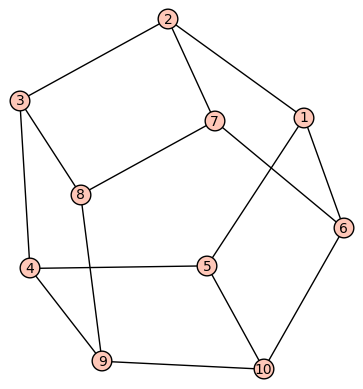
\includegraphics[width=0.5\textwidth]{prism.png}
\caption{A prism with a pentagonal base.}
\end{figure}

We now give a labeling of the arrows in the quiver associated to a prism, similar to the one we produced for pyramids, in order to help us simplify the description of the rewriting system:

\[
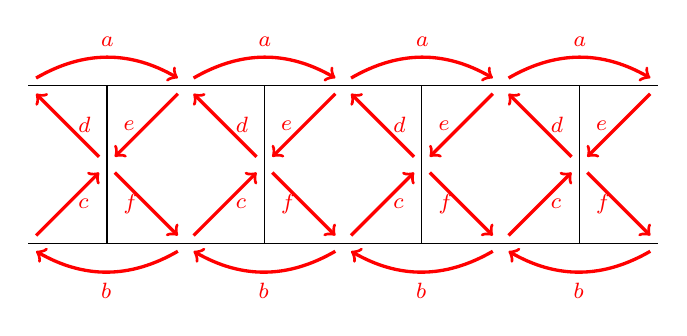
\begin{tikzpicture}[text width=1.5mm, font=\footnotesize]
\draw (-4, 0) -- (4, 0);
\draw (-4, 2) -- (4, 2);
\foreach \x in {-3,-1,...,3}
\draw (\x, 0) -- (\x, 2);
\foreach \x in {-3,-1,1}
{
\draw[->, red, very thick] (\x+1.1, 0.1) to node[right]{$c$} (\x+1.9, 0.9);
\draw[->, red, very thick] (\x+1.9, 1.1) to node[right]{$d$} (\x+1.1, 1.9);
\draw[->, red, very thick] (\x+0.9, 1.9) to node[left]{$e$} (\x+0.1, 1.1);
\draw[->, red, very thick] (\x+0.1, 0.9) to node[left]{$f$} (\x+0.9, 0.1);
}
\draw[->, red, very thick] (-5+1.1, 0.1) to node[right]{$c$} (-5+1.9, 0.9);
\draw[->, red, very thick] (-5+1.9, 1.1) to node[right]{$d$} (-5+1.1, 1.9);
\draw[->, red, very thick] (3+0.9, 1.9) to node[left]{$e$} (3+0.1, 1.1);
\draw[->, red, very thick] (3+0.1, 0.9) to node[left]{$f$} (3+0.9, 0.1);

\foreach \x in {-4,-2,...,2}
{
\draw[->, red, very thick] (\x+0.1, 2.1) to [bend left] node[above]{$a$} (\x+1.9, 2.1);
\draw[<-, red, very thick] (\x+0.1, -0.1) to [bend right] node[below]{$b$} (\x+1.9, -0.1);
}
\end{tikzpicture}
\]

We have drawn the prism as a planar figure in which the left and right sides are identified. In the drawing, the black edges represent the edges of the prism and the red arrows are the ones from the associated quiver. Arrows labeled $a$ (resp. $b$) correspond to the $n$-cycle inside the top (resp. bottom) base face. The arrows corresponding to 4-cycles inside parallelograms are labeled as $c$, $d$, $e$ or $f$, in such a way that a 4-cycle having a vertex from the top base as source is labeled $dcfe$.

After naming the arrows in this way, a confluent rewriting system for the associated Jacobian algebra in the case $n>3$ is given by the rules:
\begin{align*}
de &\rightsquigarrow -a^{n-1} 	& dcfe &\rightsquigarrow a^n \\
fc &\rightsquigarrow -b^{n-1}	& fedc &\rightsquigarrow b^n \\
ad &\rightsquigarrow -dcf		& cfed &\rightsquigarrow edcf \\
bf &\rightsquigarrow -fed  	& a^{n+1} &\rightsquigarrow 0 \\
ea &\rightsquigarrow -cfe 		& b^{n+1} &\rightsquigarrow 0 \\
cb &\rightsquigarrow -edc  	& \, & \,
\end{align*}
As one may easily check, all cycles in the quiver are reducible, except for $a^n$, $b^n$ and $edcf$. Nevertheless, all powers of these cycles are reducible, and so the Jacobian algebra is finite-dimensional. In fact, once again we may count the number of irreducible monomials of each length, which are
\begin{itemize}
\item $3n$ stationary paths,
\item $6n$ paths of lengths $k$, for $1\leq k\leq 3$,
\item $3n$ paths of length 4,
\item $2n$ paths of length $j$, for $5\leq j\leq n$.
\end{itemize}

Our second family of polyhedra is the family of \emph{antiprisms}, which are once again composed of two parallel copies of an $n$-sided polygon, but this time they are joined by triangles.

\begin{figure}[h]
\centering
	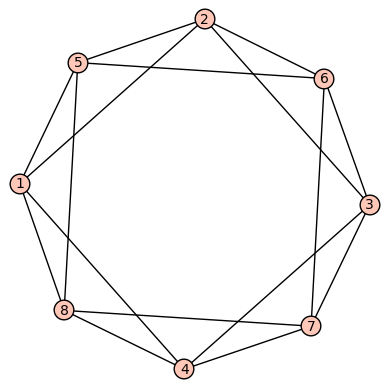
\includegraphics[width=0.5\textwidth]{antiprism.png}
\caption{Top view of an antiprism with square base.}
\end{figure}

Our labeling of the arrows in the quiver will be:


\[
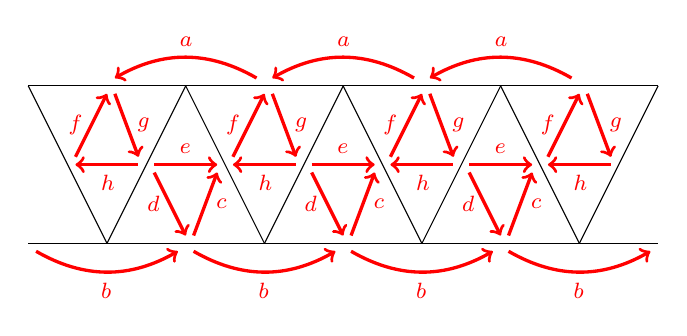
\begin{tikzpicture}[text width=1.5mm, font=\footnotesize]
\draw (-4, 0) -- (4, 0);
\draw (-4, 2) -- (4, 2);
\foreach \x in {-4,-2,...,2}
{
\draw (\x, 2) -- (\x+1, 0);
\draw (\x+1, 0) -- (\x+2, 2);
}
\foreach \x in {-3,-1,...,1}
{
\draw[<-, red, very thick] (\x+0.1, 2.1) to [bend left] node[above]{$a$} (\x+1.9, 2.1);
\draw[->, red, very thick] (\x+0.6, 1) to node[above]{$e$} (\x+1.4, 1);
\draw[->, red, very thick] (\x+0.6, 0.9) to node[left]{$d$} (\x+1, 0.1);
\draw[->, red, very thick] (\x+1.1, 0.1) to node[right]{$c$} (\x+1.4, 0.9);
}

\foreach \x in {-4,-2,...,2}
{
\draw[->, red, very thick] (\x+0.1, -0.1) to [bend right] node[below]{$b$} (\x+1.9, -0.1);
\draw[<-, red, very thick] (\x+0.6, 1) to node[below]{$h$} (\x+1.4, 1);
\draw[->, red, very thick] (\x+0.6, 1.1) to node[left]{$f$} (\x+1, 1.9);
\draw[->, red, very thick] (\x+1.1, 1.9) to node[right]{$g$} (\x+1.4, 1.1);
}
\end{tikzpicture}
\]

Once again, the polyhedron is assembled by identifying the left and right sides of the figure. Arrows labeled $a$ (resp $b$) correspond to the top (resp. bottom) $n$-cycle. Arrows inside a triangle sharing a side with the top (resp. bottom) face are labeled $f$, $g$ or $h$ (resp. $c$, $d$, $e$), in such a way that a 3-cycle having a vertex from the top (resp. bottom) face as source is labeled $fhg$ (resp. $ced$).

If $n>3$, a confluent rewriting system for the Jacobian algebra associated to an antiprism with an $n$-sided base is given by:

\begin{align*}
feg &\rightsquigarrow -a^{n-1} 	& hdbc &\rightsquigarrow egaf \\
chd &\rightsquigarrow -b^{n-1}	& gafe &\rightsquigarrow dbch \\
ed &\rightsquigarrow -hbd		& ga^{n-1} &\rightsquigarrow 0 \\
ce &\rightsquigarrow -bch  	& a^{n-1}f &\rightsquigarrow 0 \\
dc &\rightsquigarrow -gaf 		& db^{n-1} &\rightsquigarrow 0 \\
hg &\rightsquigarrow -ega  	& b^{n-1}c &\rightsquigarrow 0 \\
fh &\rightsquigarrow -afe  	& a^{2n-2} &\rightsquigarrow 0 \\
gf &\rightsquigarrow -dbc  	& b^{2n-2} &\rightsquigarrow 0 \\
\end{align*}

Although it is not as easy as with prisms, it is still straightforward to check that all squares of cycles are reducible, and therefore the Jacobian algebra turns out to be finite-dimensional as well. It is easy, although a bit tedious, to enumerate all of the irreducible monomials.\note{lo podría incluir si vale la pena, total ya lo tengo calculado} It turns out that there are
\begin{itemize}
\item $4n$ stationary paths,
\item $(6+2k)n$ irreducible paths of length $k$, for $1\leq k\leq 6$,
\item $18n$ irreducible paths of lengths $6$ to $n-1$,
\item $14n$ irreducible paths of length $n$,
\item $8n$ irreducible paths of length $n+1$,
\item $4n$ irreducible paths of length $n+2$,
\item $2n$ irreducible paths of lengths $n+3$ to $2n-3$.
\end{itemize}

As usual, we check this computation against the output of our software:
\begin{lstlisting}
sage: Rewriting_System(prism(7), True).generating_function(9)
105 rules added.
Total rules: 231
[21, 42, 42, 42, 21, 14, 14, 14, 0]

sage: Rewriting_System(antiprism(7), True).generating_function(13)
98 rules added.
48 rules added.
Total rules: 230
[28, 56, 70, 84, 98, 112, 126, 98, 56, 28, 14, 14, 0]
\end{lstlisting}
Note that we set the parameter \texttt{zero\_rules\_flag} as \texttt{True}, since there are rules in the rewriting system which are induced by the topology (namely, there are paths that reduce to zero since they may be extended to arbitrarily high lengths).
\end{section}
\end{chapter}